\documentclass[crop,tikz]{standalone}

\usepackage[utf8]{inputenc}

% 'crop' is the default for v1.0, before it was 'preview'
%\usetikzlibrary{...}% tikz package already loaded by 'tikz' option
\usetikzlibrary{arrows} 


\begin{document}

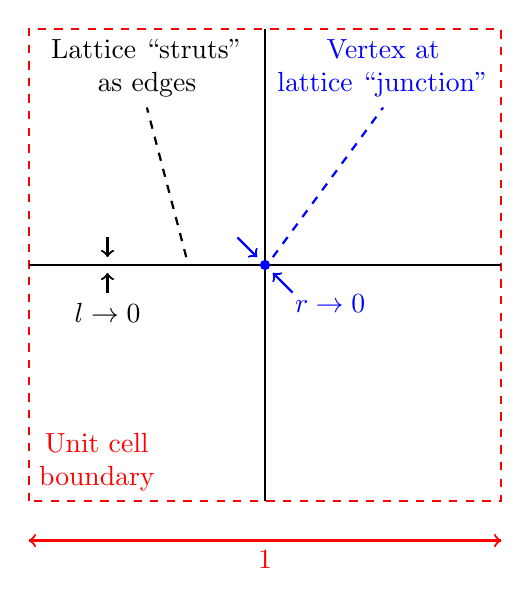
\begin{tikzpicture}[thick, main node/.style={circle,draw,font=\sffamily\Large\bfseries}]
	%periodic boundary, unit cell boundary
	\draw[dashed, red] (-3,-3) rectangle (3,3);
	\node[anchor=south west, align=center, red] at (-3,-3) {Unit cell \\ boundary};
	
	%lattice singular-structure
	\draw (-3,0) -- (3,0);
	\draw (0,-3) -- (0,3);
	
	%length scales
	%period cell size
	\draw[->, red] (-3,-3.5) -- (3,-3.5);
	\draw[->, red] (3,-3.5) -- (-3,-3.5);
	\node[anchor=north, red] at (0,-3.5) {$1$};
	
	%lattice length scale -> 0
	\draw[->] (-2,0.25+0.1) -- (-2,0+0.1);
	\draw[->] (-2,-0.25-0.1) -- (-2,0-0.1);
	\node[anchor=north] at (-2,-0.25-0.1) {$l\rightarrow0$};	
	\draw[dashed] (-1,0.1) -- (-1.5,2) node[anchor=south, align=center] {Lattice ``struts" \\ as edges};	
	
	%vertex at centre, with labels
	\draw[->, blue] (0.25+0.1, -0.25-0.1) -- (0+0.1,0-0.1);
	\draw[->, blue] (-0.25-0.1, 0.25+0.1) -- (0-0.1,0+0.1);
	\filldraw[blue] (0,0) circle ( 0.05 );
	\node[anchor=north west, blue] at (0.25,-0.25) {$r\rightarrow0$};
	\draw[dashed, blue] (0+0.1,0+0.1) -- (1.5,2) node[anchor=south, align=center] {Vertex at \\ lattice ``junction"};

\end{tikzpicture}

\end{document}